
\documentclass[10pt]{article} % For LaTeX2e
% \usepackage{tmlr}
% If accepted, instead use the following line for the camera-ready submission:
\usepackage[preprint]{tmlr}
% To de-anonymize and remove mentions to TMLR (for example for posting to preprint servers), instead use the following:
%\usepackage[preprint]{tmlr}

% Optional math commands from https://github.com/goodfeli/dlbook_notation.
%%%%% NEW MATH DEFINITIONS %%%%%

\usepackage{amsmath,amsfonts,bm}

% Mark sections of captions for referring to divisions of figures
\newcommand{\figleft}{{\em (Left)}}
\newcommand{\figcenter}{{\em (Center)}}
\newcommand{\figright}{{\em (Right)}}
\newcommand{\figtop}{{\em (Top)}}
\newcommand{\figbottom}{{\em (Bottom)}}
\newcommand{\captiona}{{\em (a)}}
\newcommand{\captionb}{{\em (b)}}
\newcommand{\captionc}{{\em (c)}}
\newcommand{\captiond}{{\em (d)}}

% Highlight a newly defined term
\newcommand{\newterm}[1]{{\bf #1}}


% Figure reference, lower-case.
\def\figref#1{figure~\ref{#1}}
% Figure reference, capital. For start of sentence
\def\Figref#1{Figure~\ref{#1}}
\def\twofigref#1#2{figures \ref{#1} and \ref{#2}}
\def\quadfigref#1#2#3#4{figures \ref{#1}, \ref{#2}, \ref{#3} and \ref{#4}}
% Section reference, lower-case.
\def\secref#1{section~\ref{#1}}
% Section reference, capital.
\def\Secref#1{Section~\ref{#1}}
% Reference to two sections.
\def\twosecrefs#1#2{sections \ref{#1} and \ref{#2}}
% Reference to three sections.
\def\secrefs#1#2#3{sections \ref{#1}, \ref{#2} and \ref{#3}}
% Reference to an equation, lower-case.
\def\eqref#1{equation~\ref{#1}}
% Reference to an equation, upper case
\def\Eqref#1{Equation~\ref{#1}}
% A raw reference to an equation---avoid using if possible
\def\plaineqref#1{\ref{#1}}
% Reference to a chapter, lower-case.
\def\chapref#1{chapter~\ref{#1}}
% Reference to an equation, upper case.
\def\Chapref#1{Chapter~\ref{#1}}
% Reference to a range of chapters
\def\rangechapref#1#2{chapters\ref{#1}--\ref{#2}}
% Reference to an algorithm, lower-case.
\def\algref#1{algorithm~\ref{#1}}
% Reference to an algorithm, upper case.
\def\Algref#1{Algorithm~\ref{#1}}
\def\twoalgref#1#2{algorithms \ref{#1} and \ref{#2}}
\def\Twoalgref#1#2{Algorithms \ref{#1} and \ref{#2}}
% Reference to a part, lower case
\def\partref#1{part~\ref{#1}}
% Reference to a part, upper case
\def\Partref#1{Part~\ref{#1}}
\def\twopartref#1#2{parts \ref{#1} and \ref{#2}}

\def\ceil#1{\lceil #1 \rceil}
\def\floor#1{\lfloor #1 \rfloor}
\def\1{\bm{1}}
\newcommand{\train}{\mathcal{D}}
\newcommand{\valid}{\mathcal{D_{\mathrm{valid}}}}
\newcommand{\test}{\mathcal{D_{\mathrm{test}}}}

\def\eps{{\epsilon}}


% Random variables
\def\reta{{\textnormal{$\eta$}}}
\def\ra{{\textnormal{a}}}
\def\rb{{\textnormal{b}}}
\def\rc{{\textnormal{c}}}
\def\rd{{\textnormal{d}}}
\def\re{{\textnormal{e}}}
\def\rf{{\textnormal{f}}}
\def\rg{{\textnormal{g}}}
\def\rh{{\textnormal{h}}}
\def\ri{{\textnormal{i}}}
\def\rj{{\textnormal{j}}}
\def\rk{{\textnormal{k}}}
\def\rl{{\textnormal{l}}}
% rm is already a command, just don't name any random variables m
\def\rn{{\textnormal{n}}}
\def\ro{{\textnormal{o}}}
\def\rp{{\textnormal{p}}}
\def\rq{{\textnormal{q}}}
\def\rr{{\textnormal{r}}}
\def\rs{{\textnormal{s}}}
\def\rt{{\textnormal{t}}}
\def\ru{{\textnormal{u}}}
\def\rv{{\textnormal{v}}}
\def\rw{{\textnormal{w}}}
\def\rx{{\textnormal{x}}}
\def\ry{{\textnormal{y}}}
\def\rz{{\textnormal{z}}}

% Random vectors
\def\rvepsilon{{\mathbf{\epsilon}}}
\def\rvtheta{{\mathbf{\theta}}}
\def\rva{{\mathbf{a}}}
\def\rvb{{\mathbf{b}}}
\def\rvc{{\mathbf{c}}}
\def\rvd{{\mathbf{d}}}
\def\rve{{\mathbf{e}}}
\def\rvf{{\mathbf{f}}}
\def\rvg{{\mathbf{g}}}
\def\rvh{{\mathbf{h}}}
\def\rvu{{\mathbf{i}}}
\def\rvj{{\mathbf{j}}}
\def\rvk{{\mathbf{k}}}
\def\rvl{{\mathbf{l}}}
\def\rvm{{\mathbf{m}}}
\def\rvn{{\mathbf{n}}}
\def\rvo{{\mathbf{o}}}
\def\rvp{{\mathbf{p}}}
\def\rvq{{\mathbf{q}}}
\def\rvr{{\mathbf{r}}}
\def\rvs{{\mathbf{s}}}
\def\rvt{{\mathbf{t}}}
\def\rvu{{\mathbf{u}}}
\def\rvv{{\mathbf{v}}}
\def\rvw{{\mathbf{w}}}
\def\rvx{{\mathbf{x}}}
\def\rvy{{\mathbf{y}}}
\def\rvz{{\mathbf{z}}}

% Elements of random vectors
\def\erva{{\textnormal{a}}}
\def\ervb{{\textnormal{b}}}
\def\ervc{{\textnormal{c}}}
\def\ervd{{\textnormal{d}}}
\def\erve{{\textnormal{e}}}
\def\ervf{{\textnormal{f}}}
\def\ervg{{\textnormal{g}}}
\def\ervh{{\textnormal{h}}}
\def\ervi{{\textnormal{i}}}
\def\ervj{{\textnormal{j}}}
\def\ervk{{\textnormal{k}}}
\def\ervl{{\textnormal{l}}}
\def\ervm{{\textnormal{m}}}
\def\ervn{{\textnormal{n}}}
\def\ervo{{\textnormal{o}}}
\def\ervp{{\textnormal{p}}}
\def\ervq{{\textnormal{q}}}
\def\ervr{{\textnormal{r}}}
\def\ervs{{\textnormal{s}}}
\def\ervt{{\textnormal{t}}}
\def\ervu{{\textnormal{u}}}
\def\ervv{{\textnormal{v}}}
\def\ervw{{\textnormal{w}}}
\def\ervx{{\textnormal{x}}}
\def\ervy{{\textnormal{y}}}
\def\ervz{{\textnormal{z}}}

% Random matrices
\def\rmA{{\mathbf{A}}}
\def\rmB{{\mathbf{B}}}
\def\rmC{{\mathbf{C}}}
\def\rmD{{\mathbf{D}}}
\def\rmE{{\mathbf{E}}}
\def\rmF{{\mathbf{F}}}
\def\rmG{{\mathbf{G}}}
\def\rmH{{\mathbf{H}}}
\def\rmI{{\mathbf{I}}}
\def\rmJ{{\mathbf{J}}}
\def\rmK{{\mathbf{K}}}
\def\rmL{{\mathbf{L}}}
\def\rmM{{\mathbf{M}}}
\def\rmN{{\mathbf{N}}}
\def\rmO{{\mathbf{O}}}
\def\rmP{{\mathbf{P}}}
\def\rmQ{{\mathbf{Q}}}
\def\rmR{{\mathbf{R}}}
\def\rmS{{\mathbf{S}}}
\def\rmT{{\mathbf{T}}}
\def\rmU{{\mathbf{U}}}
\def\rmV{{\mathbf{V}}}
\def\rmW{{\mathbf{W}}}
\def\rmX{{\mathbf{X}}}
\def\rmY{{\mathbf{Y}}}
\def\rmZ{{\mathbf{Z}}}

% Elements of random matrices
\def\ermA{{\textnormal{A}}}
\def\ermB{{\textnormal{B}}}
\def\ermC{{\textnormal{C}}}
\def\ermD{{\textnormal{D}}}
\def\ermE{{\textnormal{E}}}
\def\ermF{{\textnormal{F}}}
\def\ermG{{\textnormal{G}}}
\def\ermH{{\textnormal{H}}}
\def\ermI{{\textnormal{I}}}
\def\ermJ{{\textnormal{J}}}
\def\ermK{{\textnormal{K}}}
\def\ermL{{\textnormal{L}}}
\def\ermM{{\textnormal{M}}}
\def\ermN{{\textnormal{N}}}
\def\ermO{{\textnormal{O}}}
\def\ermP{{\textnormal{P}}}
\def\ermQ{{\textnormal{Q}}}
\def\ermR{{\textnormal{R}}}
\def\ermS{{\textnormal{S}}}
\def\ermT{{\textnormal{T}}}
\def\ermU{{\textnormal{U}}}
\def\ermV{{\textnormal{V}}}
\def\ermW{{\textnormal{W}}}
\def\ermX{{\textnormal{X}}}
\def\ermY{{\textnormal{Y}}}
\def\ermZ{{\textnormal{Z}}}

% Vectors
\def\vzero{{\bm{0}}}
\def\vone{{\bm{1}}}
\def\vmu{{\bm{\mu}}}
\def\vtheta{{\bm{\theta}}}
\def\va{{\bm{a}}}
\def\vb{{\bm{b}}}
\def\vc{{\bm{c}}}
\def\vd{{\bm{d}}}
\def\ve{{\bm{e}}}
\def\vf{{\bm{f}}}
\def\vg{{\bm{g}}}
\def\vh{{\bm{h}}}
\def\vi{{\bm{i}}}
\def\vj{{\bm{j}}}
\def\vk{{\bm{k}}}
\def\vl{{\bm{l}}}
\def\vm{{\bm{m}}}
\def\vn{{\bm{n}}}
\def\vo{{\bm{o}}}
\def\vp{{\bm{p}}}
\def\vq{{\bm{q}}}
\def\vr{{\bm{r}}}
\def\vs{{\bm{s}}}
\def\vt{{\bm{t}}}
\def\vu{{\bm{u}}}
\def\vv{{\bm{v}}}
\def\vw{{\bm{w}}}
\def\vx{{\bm{x}}}
\def\vy{{\bm{y}}}
\def\vz{{\bm{z}}}

% Elements of vectors
\def\evalpha{{\alpha}}
\def\evbeta{{\beta}}
\def\evepsilon{{\epsilon}}
\def\evlambda{{\lambda}}
\def\evomega{{\omega}}
\def\evmu{{\mu}}
\def\evpsi{{\psi}}
\def\evsigma{{\sigma}}
\def\evtheta{{\theta}}
\def\eva{{a}}
\def\evb{{b}}
\def\evc{{c}}
\def\evd{{d}}
\def\eve{{e}}
\def\evf{{f}}
\def\evg{{g}}
\def\evh{{h}}
\def\evi{{i}}
\def\evj{{j}}
\def\evk{{k}}
\def\evl{{l}}
\def\evm{{m}}
\def\evn{{n}}
\def\evo{{o}}
\def\evp{{p}}
\def\evq{{q}}
\def\evr{{r}}
\def\evs{{s}}
\def\evt{{t}}
\def\evu{{u}}
\def\evv{{v}}
\def\evw{{w}}
\def\evx{{x}}
\def\evy{{y}}
\def\evz{{z}}

% Matrix
\def\mA{{\bm{A}}}
\def\mB{{\bm{B}}}
\def\mC{{\bm{C}}}
\def\mD{{\bm{D}}}
\def\mE{{\bm{E}}}
\def\mF{{\bm{F}}}
\def\mG{{\bm{G}}}
\def\mH{{\bm{H}}}
\def\mI{{\bm{I}}}
\def\mJ{{\bm{J}}}
\def\mK{{\bm{K}}}
\def\mL{{\bm{L}}}
\def\mM{{\bm{M}}}
\def\mN{{\bm{N}}}
\def\mO{{\bm{O}}}
\def\mP{{\bm{P}}}
\def\mQ{{\bm{Q}}}
\def\mR{{\bm{R}}}
\def\mS{{\bm{S}}}
\def\mT{{\bm{T}}}
\def\mU{{\bm{U}}}
\def\mV{{\bm{V}}}
\def\mW{{\bm{W}}}
\def\mX{{\bm{X}}}
\def\mY{{\bm{Y}}}
\def\mZ{{\bm{Z}}}
\def\mBeta{{\bm{\beta}}}
\def\mPhi{{\bm{\Phi}}}
\def\mLambda{{\bm{\Lambda}}}
\def\mSigma{{\bm{\Sigma}}}

% Tensor
\DeclareMathAlphabet{\mathsfit}{\encodingdefault}{\sfdefault}{m}{sl}
\SetMathAlphabet{\mathsfit}{bold}{\encodingdefault}{\sfdefault}{bx}{n}
\newcommand{\tens}[1]{\bm{\mathsfit{#1}}}
\def\tA{{\tens{A}}}
\def\tB{{\tens{B}}}
\def\tC{{\tens{C}}}
\def\tD{{\tens{D}}}
\def\tE{{\tens{E}}}
\def\tF{{\tens{F}}}
\def\tG{{\tens{G}}}
\def\tH{{\tens{H}}}
\def\tI{{\tens{I}}}
\def\tJ{{\tens{J}}}
\def\tK{{\tens{K}}}
\def\tL{{\tens{L}}}
\def\tM{{\tens{M}}}
\def\tN{{\tens{N}}}
\def\tO{{\tens{O}}}
\def\tP{{\tens{P}}}
\def\tQ{{\tens{Q}}}
\def\tR{{\tens{R}}}
\def\tS{{\tens{S}}}
\def\tT{{\tens{T}}}
\def\tU{{\tens{U}}}
\def\tV{{\tens{V}}}
\def\tW{{\tens{W}}}
\def\tX{{\tens{X}}}
\def\tY{{\tens{Y}}}
\def\tZ{{\tens{Z}}}


% Graph
\def\gA{{\mathcal{A}}}
\def\gB{{\mathcal{B}}}
\def\gC{{\mathcal{C}}}
\def\gD{{\mathcal{D}}}
\def\gE{{\mathcal{E}}}
\def\gF{{\mathcal{F}}}
\def\gG{{\mathcal{G}}}
\def\gH{{\mathcal{H}}}
\def\gI{{\mathcal{I}}}
\def\gJ{{\mathcal{J}}}
\def\gK{{\mathcal{K}}}
\def\gL{{\mathcal{L}}}
\def\gM{{\mathcal{M}}}
\def\gN{{\mathcal{N}}}
\def\gO{{\mathcal{O}}}
\def\gP{{\mathcal{P}}}
\def\gQ{{\mathcal{Q}}}
\def\gR{{\mathcal{R}}}
\def\gS{{\mathcal{S}}}
\def\gT{{\mathcal{T}}}
\def\gU{{\mathcal{U}}}
\def\gV{{\mathcal{V}}}
\def\gW{{\mathcal{W}}}
\def\gX{{\mathcal{X}}}
\def\gY{{\mathcal{Y}}}
\def\gZ{{\mathcal{Z}}}

% Sets
\def\sA{{\mathbb{A}}}
\def\sB{{\mathbb{B}}}
\def\sC{{\mathbb{C}}}
\def\sD{{\mathbb{D}}}
% Don't use a set called E, because this would be the same as our symbol
% for expectation.
\def\sF{{\mathbb{F}}}
\def\sG{{\mathbb{G}}}
\def\sH{{\mathbb{H}}}
\def\sI{{\mathbb{I}}}
\def\sJ{{\mathbb{J}}}
\def\sK{{\mathbb{K}}}
\def\sL{{\mathbb{L}}}
\def\sM{{\mathbb{M}}}
\def\sN{{\mathbb{N}}}
\def\sO{{\mathbb{O}}}
\def\sP{{\mathbb{P}}}
\def\sQ{{\mathbb{Q}}}
\def\sR{{\mathbb{R}}}
\def\sS{{\mathbb{S}}}
\def\sT{{\mathbb{T}}}
\def\sU{{\mathbb{U}}}
\def\sV{{\mathbb{V}}}
\def\sW{{\mathbb{W}}}
\def\sX{{\mathbb{X}}}
\def\sY{{\mathbb{Y}}}
\def\sZ{{\mathbb{Z}}}

% Entries of a matrix
\def\emLambda{{\Lambda}}
\def\emA{{A}}
\def\emB{{B}}
\def\emC{{C}}
\def\emD{{D}}
\def\emE{{E}}
\def\emF{{F}}
\def\emG{{G}}
\def\emH{{H}}
\def\emI{{I}}
\def\emJ{{J}}
\def\emK{{K}}
\def\emL{{L}}
\def\emM{{M}}
\def\emN{{N}}
\def\emO{{O}}
\def\emP{{P}}
\def\emQ{{Q}}
\def\emR{{R}}
\def\emS{{S}}
\def\emT{{T}}
\def\emU{{U}}
\def\emV{{V}}
\def\emW{{W}}
\def\emX{{X}}
\def\emY{{Y}}
\def\emZ{{Z}}
\def\emSigma{{\Sigma}}

% entries of a tensor
% Same font as tensor, without \bm wrapper
\newcommand{\etens}[1]{\mathsfit{#1}}
\def\etLambda{{\etens{\Lambda}}}
\def\etA{{\etens{A}}}
\def\etB{{\etens{B}}}
\def\etC{{\etens{C}}}
\def\etD{{\etens{D}}}
\def\etE{{\etens{E}}}
\def\etF{{\etens{F}}}
\def\etG{{\etens{G}}}
\def\etH{{\etens{H}}}
\def\etI{{\etens{I}}}
\def\etJ{{\etens{J}}}
\def\etK{{\etens{K}}}
\def\etL{{\etens{L}}}
\def\etM{{\etens{M}}}
\def\etN{{\etens{N}}}
\def\etO{{\etens{O}}}
\def\etP{{\etens{P}}}
\def\etQ{{\etens{Q}}}
\def\etR{{\etens{R}}}
\def\etS{{\etens{S}}}
\def\etT{{\etens{T}}}
\def\etU{{\etens{U}}}
\def\etV{{\etens{V}}}
\def\etW{{\etens{W}}}
\def\etX{{\etens{X}}}
\def\etY{{\etens{Y}}}
\def\etZ{{\etens{Z}}}

% The true underlying data generating distribution
\newcommand{\pdata}{p_{\rm{data}}}
% The empirical distribution defined by the training set
\newcommand{\ptrain}{\hat{p}_{\rm{data}}}
\newcommand{\Ptrain}{\hat{P}_{\rm{data}}}
% The model distribution
\newcommand{\pmodel}{p_{\rm{model}}}
\newcommand{\Pmodel}{P_{\rm{model}}}
\newcommand{\ptildemodel}{\tilde{p}_{\rm{model}}}
% Stochastic autoencoder distributions
\newcommand{\pencode}{p_{\rm{encoder}}}
\newcommand{\pdecode}{p_{\rm{decoder}}}
\newcommand{\precons}{p_{\rm{reconstruct}}}

\newcommand{\laplace}{\mathrm{Laplace}} % Laplace distribution

\newcommand{\E}{\mathbb{E}}
\newcommand{\Ls}{\mathcal{L}}
\newcommand{\R}{\mathbb{R}}
\newcommand{\emp}{\tilde{p}}
\newcommand{\lr}{\alpha}
\newcommand{\reg}{\lambda}
\newcommand{\rect}{\mathrm{rectifier}}
\newcommand{\softmax}{\mathrm{softmax}}
\newcommand{\sigmoid}{\sigma}
\newcommand{\softplus}{\zeta}
\newcommand{\KL}{D_{\mathrm{KL}}}
\newcommand{\Var}{\mathrm{Var}}
\newcommand{\standarderror}{\mathrm{SE}}
\newcommand{\Cov}{\mathrm{Cov}}
% Wolfram Mathworld says $L^2$ is for function spaces and $\ell^2$ is for vectors
% But then they seem to use $L^2$ for vectors throughout the site, and so does
% wikipedia.
\newcommand{\normlzero}{L^0}
\newcommand{\normlone}{L^1}
\newcommand{\normltwo}{L^2}
\newcommand{\normlp}{L^p}
\newcommand{\normmax}{L^\infty}

\newcommand{\parents}{Pa} % See usage in notation.tex. Chosen to match Daphne's book.

\DeclareMathOperator*{\argmax}{arg\,max}
\DeclareMathOperator*{\argmin}{arg\,min}

\DeclareMathOperator{\sign}{sign}
\DeclareMathOperator{\Tr}{Tr}
\let\ab\allowbreak


\usepackage{hyperref}
\usepackage{url}
\usepackage{amsthm}
\usepackage{graphicx}


\newtheorem{theorem}{Theorem}


\title{A simple and efficient method for PMF estimation}

% Authors must not appear in the submitted version. They should be hidden
% as long as the tmlr package is used without the [accepted] or [preprint] options.
% Non-anonymous submissions will be rejected without review.

% \author{\name Alex Shtoff \email alexander.shtoff@tii.ae \\ Technology Innovation Institute\\}
\author{\name Alex Shtoff \email alex.shtof@gmail.com}

% The \author macro works with any number of authors. Use \AND 
% to separate the names and addresses of multiple authors.

\newcommand{\fix}{\marginpar{FIX}}
\newcommand{\new}{\marginpar{NEW}}

\def\month{MM}  % Insert correct month for camera-ready version
\def\year{YYYY} % Insert correct year for camera-ready version
\def\openreview{\url{https://openreview.net/forum?id=XXXX}} % Insert correct link to OpenReview for camera-ready version

\DeclareMathOperator{\diag}{diag}

\begin{document}


\maketitle

\begin{abstract}
We introduce a \emph{simple}, \emph{fast}, and \emph{interpretable} non-parametric method to smooth histograms and estimate a probability mass function (PMF) on $[N] = \{0,1, \dots, N - 1\}$. The core idea is to treat the empirical counts as a signal on a line graph and apply a data-dependent low-pass filter. Concretely, we form a symmetric tri-diagonal operator $\mH = \mL - \diag(\vv)$—the path graph Laplacian $\mL$ plus a diagonal bias $\vv$ built from the empirical counts—and then keep only the first $k$ eigenvectors, corresponding to the smallest eigenvalues. Projecting the empirical histogram onto this $k$-dimensional subspace produces a smooth, multi-modal estimate that preserves coarse structure while suppressing noise. A light post-processing step of clipping and re-normalizing produces a valid PMF. Moreover, we show that $k$ has an intuitive meaning - it roughly corresponds to an upper bound on the number of modes we expect the distribution to have. 

Since our main computational workhorse is computing eigenpairs of a symmetric tridiagonal matrix, we stand on the shoulders of the giants who devised and implemented fast and extremely reliable solvers (e.g., \texttt{scipy.linalg.eigh\_tridiagonal}) that run in $O(kN)$ time and $O(N)$ memory for a PMF over $[N]$. Thus, our method scales linearly with $N$, and requires no monitoring and almost no tuning. Thus our method is a principled, transparent, and fast PMF estimator that is easy to implement, tune, and explain.

\end{abstract}

\section{Introduction}
Estimating a densities from empirical observations is a fundamental problem with applications ranging from visualizing a histogram to complex generative models for images and text. In this work we focus on an extremely simple and fundamental instance - estimating the density of a discrete random variable with support in $[N] = \{0, 1, 2, \ldots, N - 1\}$ from empirical observations. Our primary focus is on a large $N$, between thousands and a few millions, where the density being estimated is multi-modal and ``heavy tailed'' densities. The quotations are because we do not mean heavy tailedness in the classical sense, due to the finite support, but we do mean that a large portion of their mass is spread far away from a small number of areas of concentration.

Examples include, but not limited to, the well-known power-law distributions, such as the Zipf distributions $p(n)\propto (a+n)^{-b}$, their centered variants $p(n) \propto (a + |n - \mu|)^{-b}$, and their mixtures. Such distributions can be naturally obtained from counts, such as token counts in a corpus of documents in the language domain, or the number of page visits in the recommender systems domain. Moreover, high resolution discretizations of continuous quantities, such as the time since the last user interaction with a given item, product prices, network latencies, or ad auction bids also yield similar density families, since the underlying continuous distributions are typically heavy-tailed.

The two most commonly employed univariate density estimators are binned empirical frequencies \citep{binning_pearson}, and kernel density estimation \citep{kde_parzen,kde_rosenblatt}. Both are extensively used in standard data visualization libraries, such as Matplotlib \citep{matplotlib} and Seaborn \citep{seaborn}. However, for heavy-tailed distributions it's hard to determine the right placement of bins to get both a reasonable and aesthetically pleasing distribution, whereas with Kernel density estimator one must set the right kernel and its width hyperparameters, which may be challenging and non-intuitive. 

At first glance, a reasonable estimation technique would be attempting to estimate the density as a mixture of centered Zipf-like distributions described above, i.e., a mixture of atoms of the form $p_i(n) \propto (a_i + |n - \mu_i|)^{-b_i}$ for $i = 1, \dots, K$, where $K$ is a reasonable upper-bound on the number of modes. Alternatively, we may try a kernel-density estimator whose kernel is of the above form, centered around the data points. In the mixture case, fitting the atom parameters together with the mixture weights is a challenging numerical task. Moreover, the actual data may behave differently from this (or any other) parametric model, such as being non-symmetrically spread around the modes. In the case of kernel density, we are not aware of a reasonable heuristic to choose the right hyper-parameters quickly and reliably, and these hyper-parameters are meaningless to a domain expert that may not be well-versed in mathematics.

We believe that a fundamental and extremely simple problem deserves an extremely simple solution. Thus, our main contribution is a simple, non-parametric, and fast method that fits heavy-tailed densities well, and is reliable to compute without tuning or oversight. 

After a short literature review in \Secref{sec:review}, we first present our method in \Secref{sec:method}, and demonstrate its strengths and weaknesses with a few synthetic distributions. Then, in \Secref{sec:analysis} we analyze it mathematically, draw a relationship with related methods from other scientific disciplines, and motivate the meaning of its only hyperparameter, the number of eigen-pairs, as an upper bound on the expected number of modes. Finally, in \Secref{sec:experiments} we demonstrate our method on several data-sets, showing both where it shines and where it does not. The somewhat nonstandard structure, where we show results of experiments on synthetic examples outside of a dedicated experiments section was chosen on purpose, since we believe this is the right way to understand our method.

\section{Previous work}\label{sec:review}
TODO - literature review. Remind older papers from computer graphics. Talk about mixture estimators and kernel density estimators in general. Say that our method doesn't require complex numerical algorithms and doesn't rely on vague convergence guarantee or specifying non-intuitive hyperparameters in contrast to these.

Talk about Laplacian and Schrodinger eigenmaps. Say that our method is a direct application of these general techniques to density estimation, treating the integers as a path graph, and the empirical frequencies as the potential in order to fit spiky heavy-tailed PMFs. Cite papers both from computer graphics and machine learning. Give proper credit to both fields.

\section{Our method}\label{sec:method}
To describe our method, we denote by $\Delta_N$ the $N$-dimensional probability simplex, by $[x]_+ = \max(x, 0)$ the positive-part function, and by $\mL$ the \emph{Laplacian} matrix
\begin{equation}\label{eq:laplacian}
\mL =\begin{pmatrix}
    1 & -1 & 0 & 0 & \cdots & 0 \\
    -1 & 2 & -1 & 0 & \cdots & 0 \\
    0 & -1 & 2 & -1 & \cdots & 0 \\
    \vdots & \vdots & \ddots & \ddots & \ddots & \vdots \\
    0 & 0 & \cdots & -1 & 2 & -1 \\
    0 & 0 & \cdots & 0 & -1 & 1
    \end{pmatrix},
\end{equation}
which lies at the heart of our method. Note, that $\mL$ is symmetric and tridiagonal.

Having observed samples from $[N]$, the inputs to our method are the vector $\vp \in \Delta_N$ of the empirical sample frequencies, and a small integer $k \in \sN$, e.g., $k = 10$. The method consists of the following four steps:
\begin{enumerate}
\item Form the symmetric and tri-diagonal matrix $\mH = \mL - \diag(\vp)$.
\item Compute the $k$ eigenvectors $\vv_1, \dots, \vv_k$ corresponding to the \emph{smallest} eigenvalues of $\mH$, and place them in the columns of the matrix $\mV = [\vv_1 \vert \vv_2 \vert \cdots \vert \vv_k]$.
\item Compute $\vu = \mV (\mV^T \vp)$
\item Return the vector $\vp$ with $\evp_i = [u_i]_+ / \| [\vu]_+ \|_1$.
\end{enumerate}
At first glance it may not be obvious why those four steps. Readers may notice that that the third step is merely a projection onto the subspace spanned by the eigenvectors, whereas the fourth step is just a normalization. Consequently, the utility of this specific subspace is the main pillar of our method's fitting performance, whereas having the reliable and efficient tools to compute the eigenvectors is the main pillar of our method's efficiency and reliability.

But before taking a closer look, we would like to draw the readers' attention to Figure \ref{fig:apx_synthetic}, where we demonstrate using synthetic examples where our method shines versus where it does not. It is apparent that ``spiky'' distributions having significant mass both around their modes but also far away are fit well, whereas Gaussian kernel-density estimation falls short. Our method is slighly less suited to wide bell-shaped distributions, in contrast to Gaussian kernel-density estimation that shines in these cases. Finally, our method performs poorly for discontinuous densities, in contrast to kernel-density estimators that, despite fitting poorly, performs gracefully. Our analysis in the next section attempts to explain these empirical phenomena.

\section{The meaning of the eigenvectors}\label{sec:analysis}
Although our method is a straightforward instance of Schr\"odinger eigenmaps, and we could simply cite that literature, we present a direct, elementary analysis to offer clearer insight and broader accessibility. We rely only on basic linear algebra facts, and adopt the viewpoint of optimizing an objective that balances data fitting and regularization, the bread and butter of modern machine learning. Some steps may be routine for readers familiar with related techniques, but this elementary treatment, in our view, makes the key ideas accessible to a much wider audience.

Recall that any real symmetric matrix always has real eigenvalues, and the corresponding eigenvectors form an orthonormal set. A well-known characterization of the eigenvalues and eigenvectors of symmetric matrices is via minimization of quadratic functions. Formally, we have:
\begin{theorem}\label{thm:courant_fischer}
Let $\mA$ be a real symmetric $n \times n$ matrix, let $\lambda_1 \leq \dots \leq\lambda_n$ be its eigenvalues, and let $\ve_1, \dots, \ve_n$ be the corresponding normalized eigenvectors. Then,
\[
\ve_k = \argmin_{\vx} \{ \vx^T \mA \vx : \|\vx\|_2 = 1,~\vx^T \ve_1 = 0,~\ldots,~\vx^T \ve_{k-1} = 0 \}.
\]
\end{theorem}
In other words, the eigenvector corresponding to the $k$-th smallest eigenvalue is the unit-norm minimizer the quadratic function $\vx^T \mA \vx$ that is orthogonal to all previous eigenvectors. Even though it is not stated in this form in the literature, this claim typically appears \emph{inside} proofs of the famous Courant-Fischer theorem. See, e.g., proof of Theorem 4.2.8 in \citet{horn2012matrix}.

Now we shall analyze our method. Consider the matrix $\mH = \mL - \diag(\vp)$, where $\mL$ is the Laplacian defined in \eqref{eq:laplacian}, and $\vp$ is the vector of empirical frequencies. By Theorem \ref{thm:courant_fischer}, the eigenvector corresponding to its smallest eigenvalue minimizes the function
\[
\vx^T (\mL - \diag(\vp)) \vx = \vx^T \mL \vx - \vx^T \diag(\vp) \vx = \underbrace{\vx^T \mL \vx}_{(*)} + \underbrace{\langle \vx^2, -\vp \rangle}_{(**)},
\]
where $\vx^2$ denotes component-wise squaring. To grasp the meaning of $(*)$, consider a variant of the difference matrix
\[
\mD = \begin{pmatrix}
    1 & -1 & 0 & \dots & 0 \\
    0 & 1 & -1 & \dots & 0 \\
    \vdots &   & \ddots & \ddots \\
    0 & \dots & 0 & 1 & -1 \\
    0 & \dots & 0 & 0 & 0
\end{pmatrix}.
\]
It is easy to verify that $\mL = \mD^T \mD$. Therefore,
\[
(*) = \vx^T \mL \vx = \| \mD \vx \|^2,
\]
meaning that this is a smoothness term penalizing the squared-norm of the differences between adjacent components of $\vx$. In other words, it is a \emph{regularizer}, and imposes a non-parametric prior of $\vx$ representing a sequence that changes slowly.

The term $(**)$ may appear familiar to machine-learning practitioners - it is the widely used inner-product similarity measure between the vectors $\vx^2$ and $\vp$. It penalizes misalignment between these two vectors, and thus serves as the alignment term between $\vx$ and the empirical frequency.

Intuitively, the first eigenvector just minimizes the balance between these two terms, and thus yields a smooth sequence that captures the over-all shape of the density. The second eigenvector aims to minimize the same balance while being orthogonal to the first, thus it may capture additional more intricate details that were not captured by the first. This pattern repeats for all eigenvectors, each capturing additional details that the previous did not. 

Figure \figref{fig:eigenvectors} demonstrates the eigenvectors obtained from samples coming from various synthetic distributions. We can observe empirically that in a multi-modal distribution, the first eigenvector typically captures the most dominant mode: the data alignment term draws the eigenvector towards the mode, whereas the smoothness penalty makes it discard other less dominant modes. Having captured all dominant modes, the remaining eigenvectors appear as oscillating sequences with increased frequency, with oscillations mostly concentrating around the modes.

This phenomenon is not a coincidence. The eigenvectors of the Laplacian matrix $\mL$ itself are the celebrated Discrete Cosine Transform \citep{the_dct}, which are renowned for their ability to approximate discrete smooth signals using a linear combination of just a few vectors. In contrast to the discrete cosine transform, which is a data-independent basis, the eigenvectors $\vv_1, \dots, \vv_k$ we use in our method are a \emph{data-dependent} basis for smooth approximations. It concentrates its approximation power in a way that is aligned with how the data is distributed.

\begin{figure}[tbh]
    \centering
    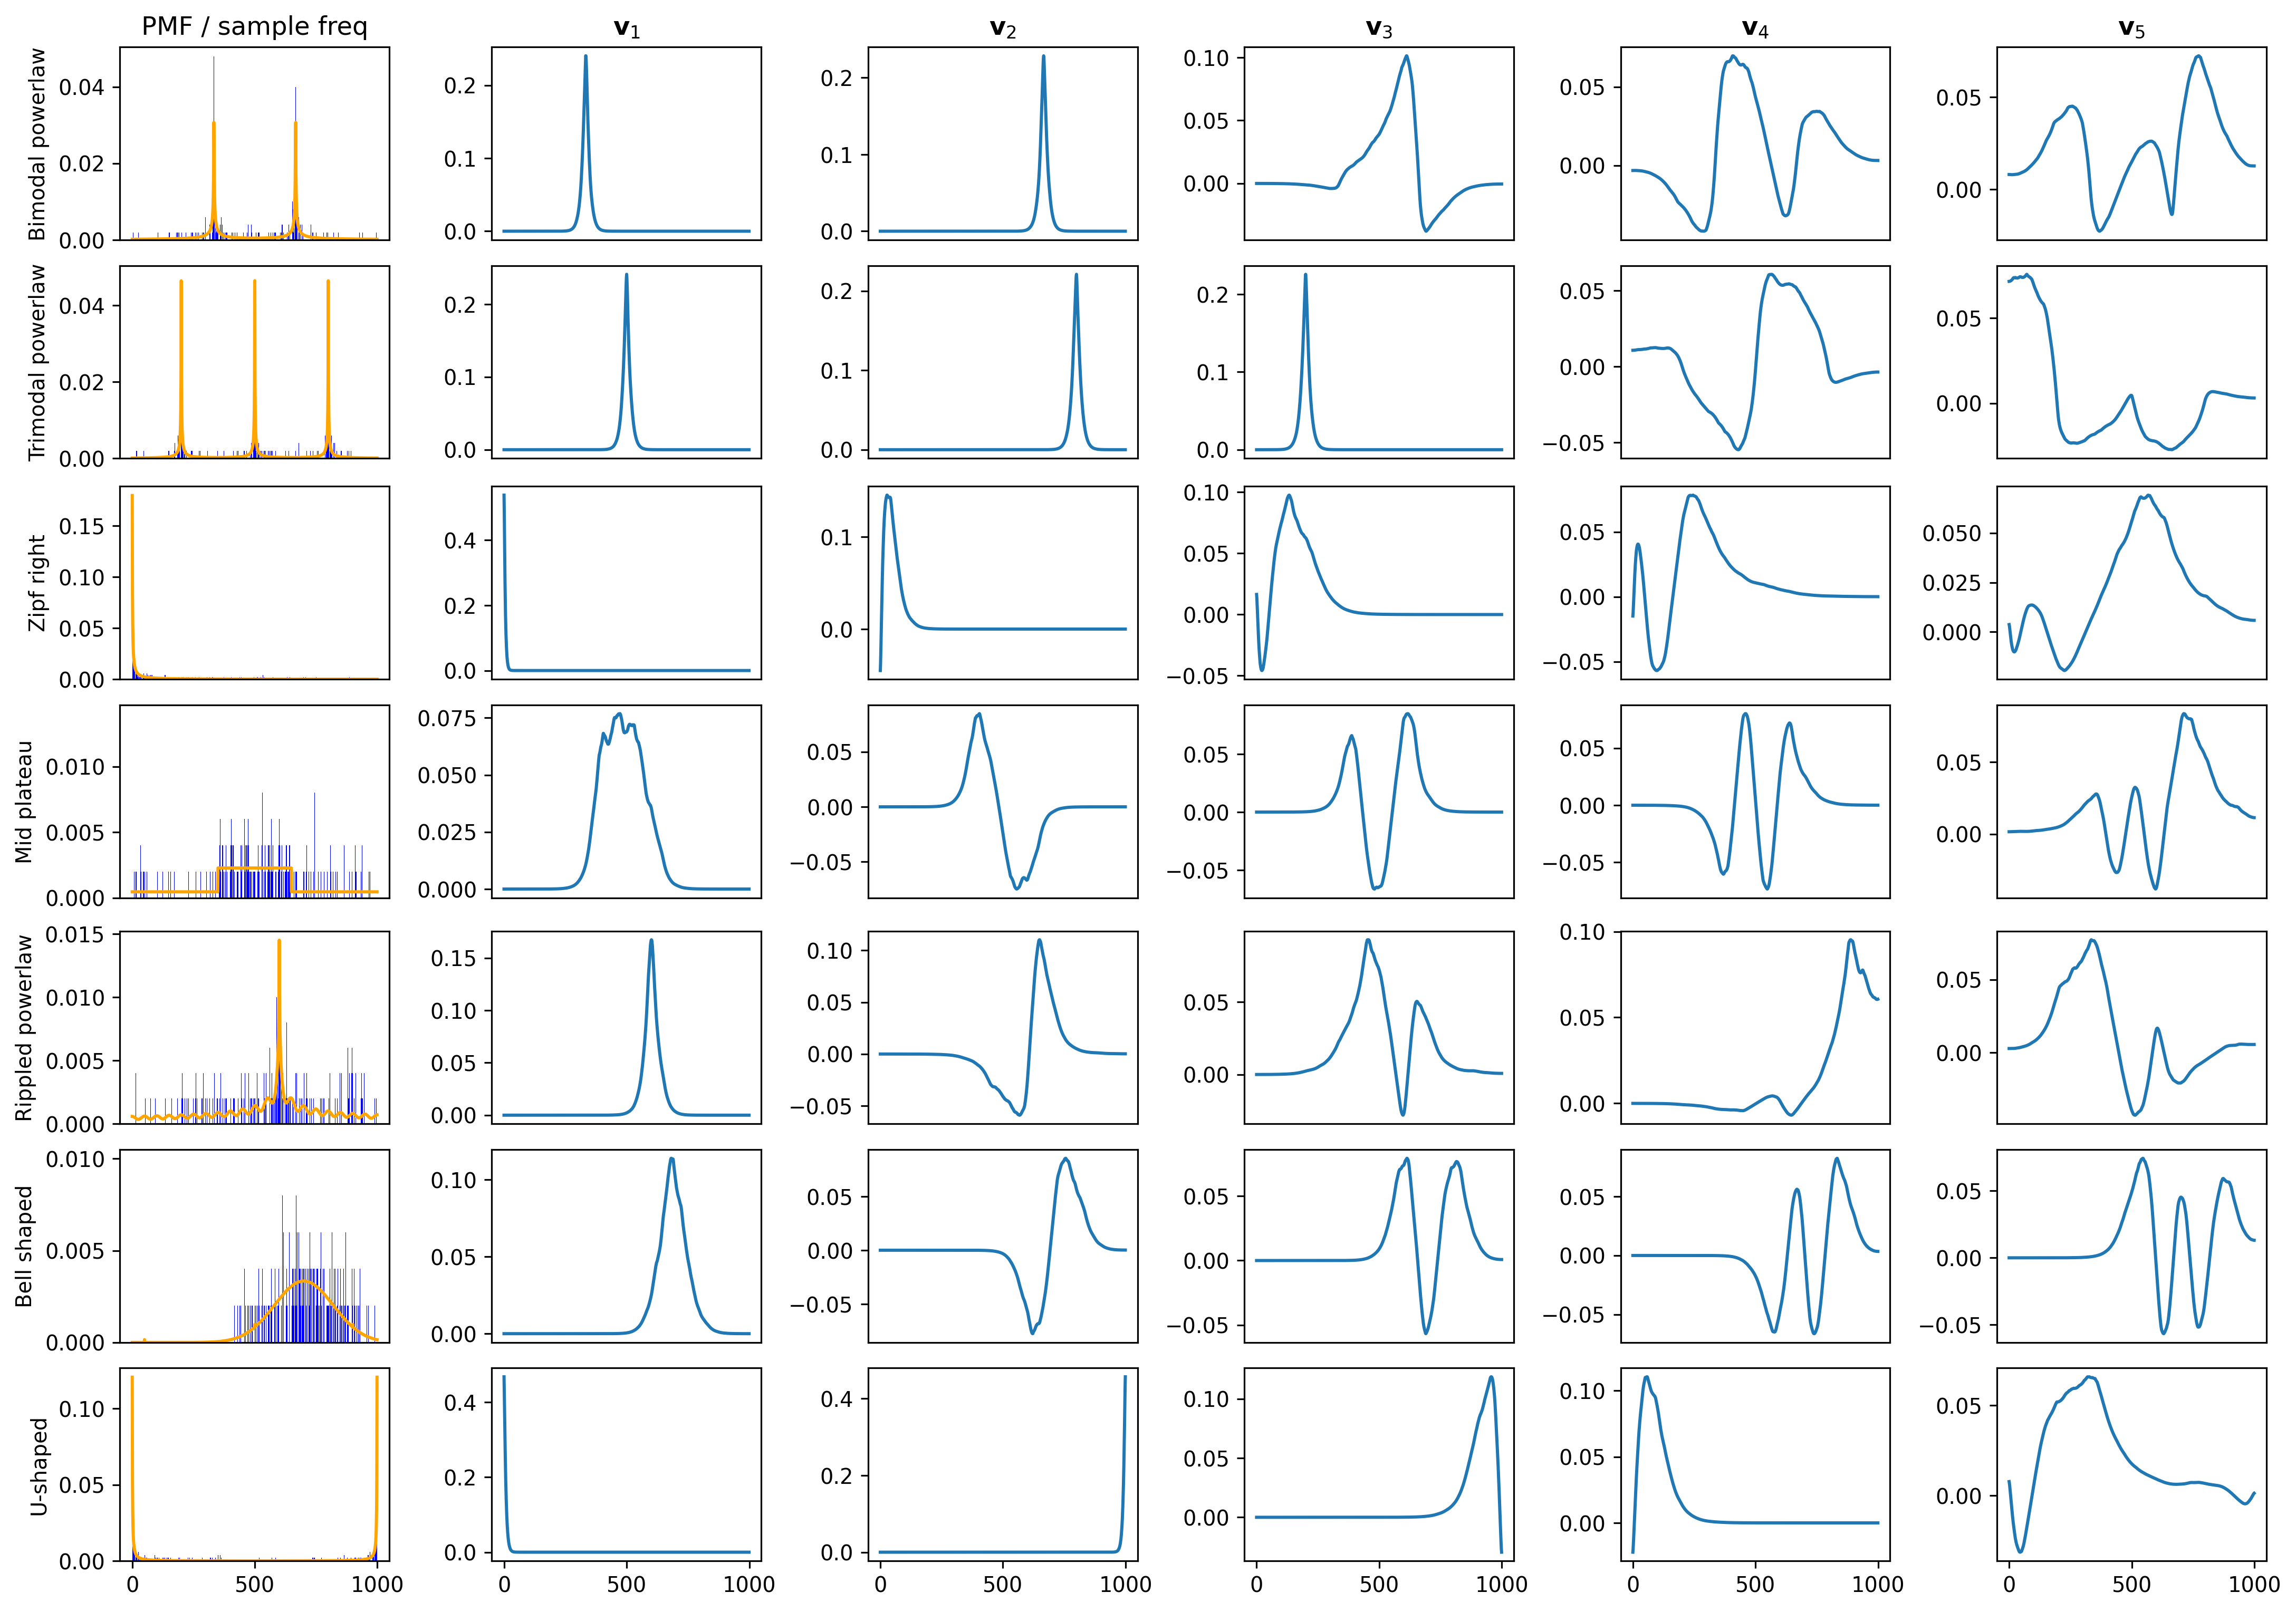
\includegraphics[width=\textwidth]{eigenvectors}
    \caption{PMFs, samples, and eigenvectors. The left-most column has the true PMF supported on $0, 1, \dots, 999$ in orange, and empirical frequencies $\vp$ obtained from 500 samples in blue. The next columns depict the first five eigenvectors of $\mL - \diag(\vp)$.}
    \label{fig:eigenvectors}
\end{figure}

\Figref{fig:apx_synthetic} continues \figref{fig:eigenvectors}, and depicts the projections of the empirical frequencies onto the space spanned by the first $k$ eigenvectors, for various values of $k$ and two sample sizes. As is apparent, the spiky shape of the heavy-tailed mixtures is nicely captured by the projection. In contrast, a bell-shaped distribution is poorly captured, even with 10 eigenvectors. A distribution with an abruptly changing PMF, the ``Mid plateau'', is a case when our method fails. Moreover, frequencies coming from densities having $k$ spikes are well approximated by roughly $k$ eigenvectors. This reinforces the interpretation of $k$ as, roughly, an upper bound on the expected number of modes. However, wide 

\begin{figure}[tbh]
    \centering
    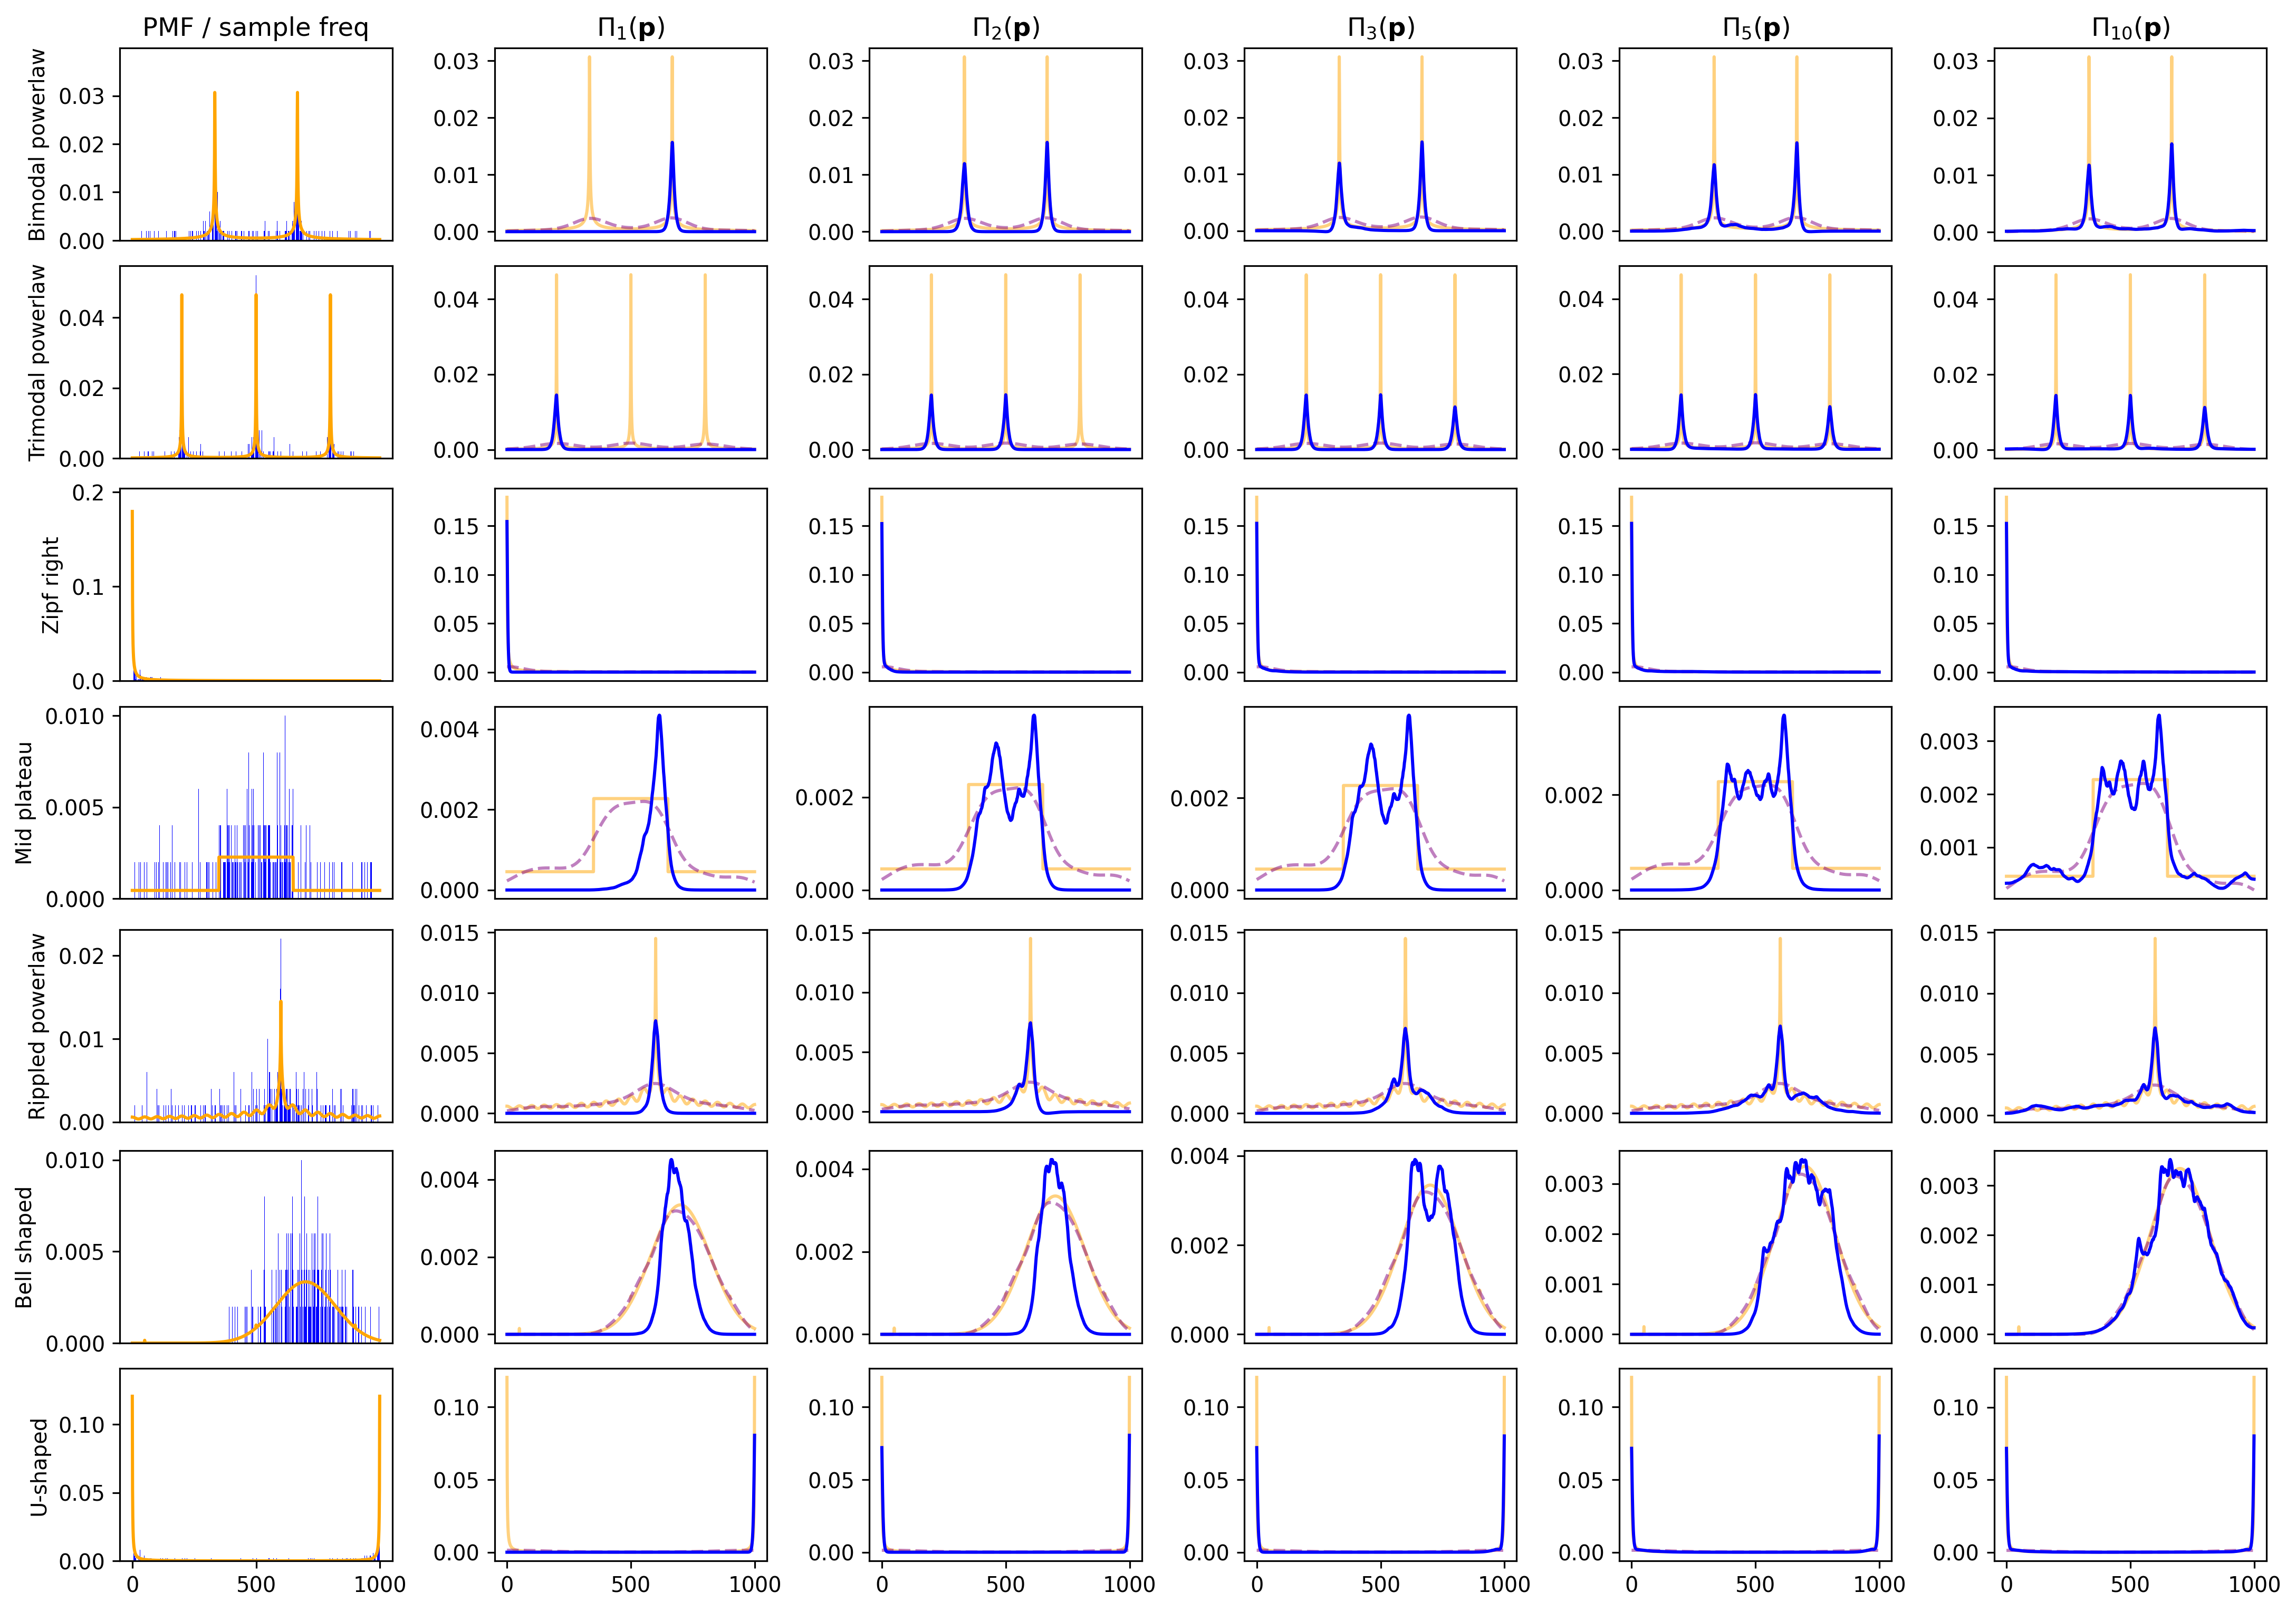
\includegraphics[width=\textwidth]{proj_500_samples}
    \caption{The projections of the empirical frequencies stemming from 500 samples from $\{0, 1, \dots, 999\}$ onto the first $k$ eigenvectors of $\mL - \diag(\vp)$ for different values of $k$. Rows are various distribution shapes. The first column depicts the empirical histogram along with the true PMF. The next columns depict projections of this empirical frequency vector onto eigenspaces of increasing dimension in blue, the kernel-density estimator obtained by calling \texttt{scipy.stats.
gaussian\_kde} in purple, and the true density in yellow.}
    \label{fig:apx_synthetic}
\end{figure}

To appreciate how our method scales with various sample sizes, we plot the projection onto the first $k=10$ eigenvectors the empirical frequency vectors coming from increasingly large samples in \figref{fig:apx_sample_sizes}. The same behavior persists - the shape of spiky distributions is nicely captured even with a small number of samples. A bell-shaped distribution requires more samples to capture, whereas kernel density-estimation works well even with small samples. And finally, our method is poorly suited in the case of an abruptly changing PMF, the ``Mid plateau''. In contrast, in this case kernel-density estimation, even though it is unable to capture the shape correctly, behaves quite gracefully.

\begin{figure}[tbh]
    \centering
    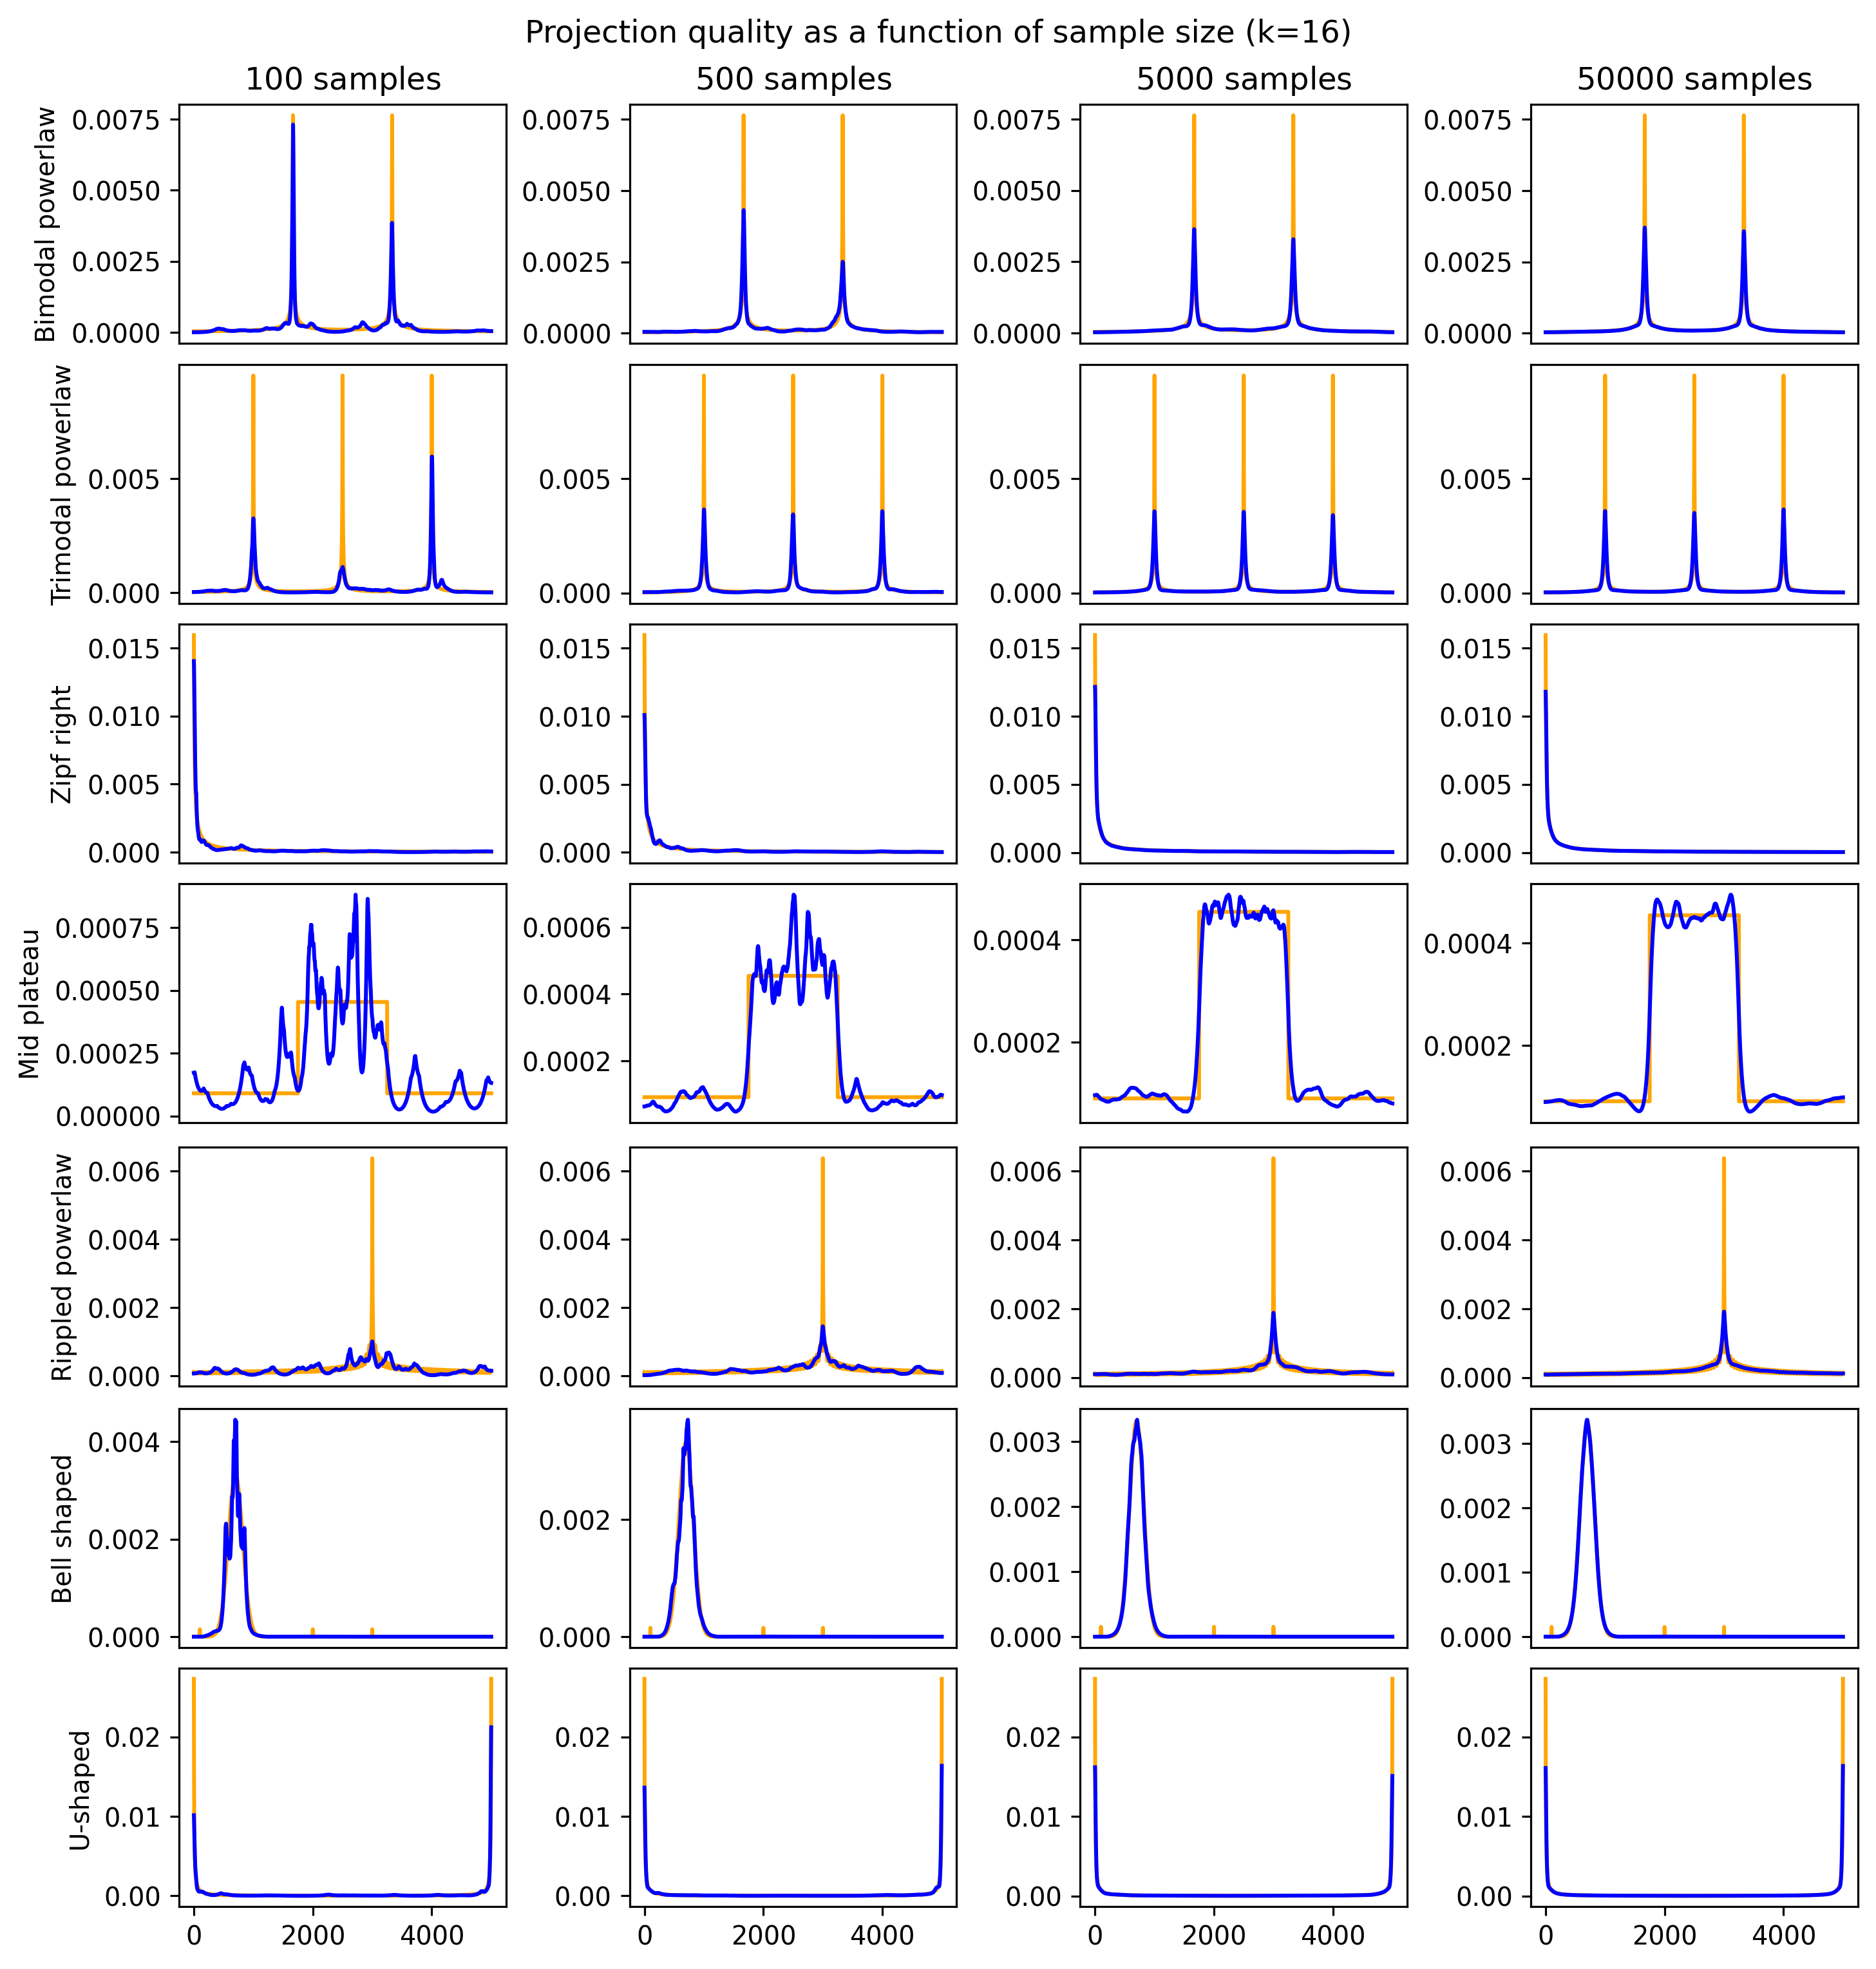
\includegraphics[width=\textwidth]{proj_diff_samples.png}
    \caption{The projections of the empirical histograms stemming from  samples from $\{0, 1, \dots, 999\}$ of various sizes onto the first $k=10$ eigenvectors of $\mL - \diag(\vp)$. Rows are various distribution shapes. Columns represent sample sizes. Our method in blue, the kernel-density estimator obtained by calling \texttt{scipy.stats.
    gaussian\_kde} in purple, and the true density in yellow.}
    \label{fig:apx_sample_sizes}
\end{figure}


\section{Summary and discussion}
The method we proposed in this paper is simple, fast, and has a reasonably intuitive hyperparameter - the expected number of modes. However, it is extremely basic, and lacks any theoretical guarantee.

It is possible that a better method, with guarantees, can be devised by a different matrix that is not necessarily the Laplacian, or by choosing a different diagonal perturbation that is not necessarily the vector of empirical frequencies. In this manuscript, we do not attempt to suggest that our method is optimal in some sense, only that it's a viable alternative for PMF estimation in an interesting case when the "go-to" method fails.

However, we hope we have inspired researchers into looking for better methods along the lines presented in this paper, and that we have made the idea of constructing a data-dependent basis more accessible to the ML audience.

\bibliography{tmlr}
\bibliographystyle{tmlr}


\end{document}
